\documentclass[12pt]{article}
\usepackage[margin=.8in, top=0.5in]{geometry}
\usepackage[all]{nowidow}
\usepackage[hyperfigures=true, hidelinks, pdfhighlight=/N]{hyperref}
\usepackage[separate-uncertainty=true, group-digits=false]{siunitx}
\usepackage{graphicx,amsmath,physics,tabto,float,amssymb,pgfplots,verbatim,tcolorbox}
\usepackage{listings,xcolor,subfig,caption,import,wrapfig,lipsum,pdfpages,eso-pic}
\usepackage{atbegshi,pdflscape,ifthen,calc,appendix}
\usepackage[version=4]{mhchem}
\numberwithin{equation}{section}
\numberwithin{figure}{section}
\numberwithin{table}{section}
\definecolor{stringcolor}{HTML}{C792EA}
\definecolor{codeblue}{HTML}{2162DB}
\definecolor{commentcolor}{HTML}{4A6E46}
\lstdefinestyle{appendix}{
    basicstyle=\ttfamily\footnotesize,commentstyle=\color{commentcolor},keywordstyle=\color{codeblue},
    stringstyle=\color{stringcolor},showstringspaces=false,numbers=left,upquote=true,captionpos=t,
    abovecaptionskip=12pt,belowcaptionskip=12pt,language=Python,breaklines=true,frame=single}
\lstdefinestyle{inline}{
    basicstyle=\ttfamily\footnotesize,commentstyle=\color{commentcolor},keywordstyle=\color{codeblue},
    stringstyle=\color{stringcolor},showstringspaces=false,numbers=left,upquote=true,frame=tb,
    captionpos=b,language=Python}
\renewcommand{\lstlistingname}{Appendix}
\pgfplotsset{compat=1.17}

\begin{document}

\begin{center}
    {\huge Poisson Statistics Analysis}\\
    \vspace{0.2in}
    \textbf{May 2021}

    \section*{Abstract}
    We test the hypothesis that count data from a Geiger counter detecting radiation from a \ce{^{60}Co} source follows a Poisson distribution. This includes deriving the equations for quantities that describe the distribution, such as mean and variance. 

\end{center}

\section{Introduction}\label{sec:Introduction}
\par The underlying goal of any experiment is to collect data on some phenomenon or process and decide, by some rigorous mathematical method, whether or not the data supports the theory describing that phenomenon or process. Theory often predicts outcomes to an exact precision, but due to the nature of measurement, experiments will never be able to exactly confirm theories, they will only ever be able to agree within an accepted experimental uncertainty. The method by which these uncertainties are estimated is explored in this experiment, as well as some implementation of those methods to attempt to confirm a hypothesis. 
\par The hypothesis in question is that the ionising radiation emitted by some radioactive source is emitted with a varying frequency that is distributed according to a Poisson distribution. We will test this hypothesis by using a Geiger counter to see a representation of the amount of radiation emitted in a given time period and then using some mathematical methods, outlined in the first part of \autoref{sec:Analysis}, to test whether this data actually follows a Poisson distribution.

\section{Method}\label{sec:Method}
\par Due to the limitations of equipment, we are not able to detect every single emission from the source but since there is no bias for radiation to be emitted in a certain direction, we can simply place our detector, a Geiger counter, pointing at the source and this should give a representative sample of the emitted radiation. Since we are not concerned with the quantitative data, such as number of emissions per second, but only with the qualitative distribution of the data this limitation is no issue. 
\par We began by letting the Geiger counter run for 10 seconds, 100 times, with no radioactive source nearby in order to determine the background radiation in the lab. After this we retrieved our \ce{^{60}Co} source and placed it in front of the Geiger counter. We wanted to analyse the data from multiple approximate count rates or frequencies: 4/10s, 10/10s, 30/10s, and 100/10s. To achieve different rates the source could be moved closer to or further away from the Geiger counter.
\par Each student was assigned a count rate from the 3 higher rates and we shared our data among ourselves in order to have a complete set, as well as used the example data supplied for the 4/10s count rate. For each rate we ran the experiment for 100 trials of 10 seconds each.

\section{Analysis}\label{sec:Analysis}
\par Our sample of \ce{^{60}Co} has a number of nuclei on the order of Avagadro's number, $\sim 10^{23}$, and since the half life of \ce{^{60}Co} is 5.27 years \cite{manual} while the time taken collecting data was around 30 minutes, the total number of nuclei throughout the course of the experiment was approximately constant: $N_n$. The number of nuclei that decay in any one time step is in general given by the binomial distribution $B(n;p,N_n)$ but since in our case $N_n$ is huge and $p$ is tiny, we can safely approximate this distribution by the Poisson distribution $P(n;\mu)$, where $\mu=pN_n$ (). To justify this, we can compute the probability $p$ of any one nucleus decaying during one trial of 10 seconds:
\par The probability that any one nucleus will decay in a trial of length 5.27 years is 0.5. Thus the probability that any one nucleus will decay in a trial of length 10 seconds is
\begin{align*}
    p&=0.5\frac{10s}{5.27y}\\
    &=0.5\frac{10s}{166308552s}\\
    &=\num{3.006e-8}
\end{align*}
\par Since the Poisson distribution gives $p=\frac{\mu}{N_n}$ and $N_n$ is very large, $p$ being of order $\num{1e-8}$ is reasonable. 
\par Our assumption is that the data we have collected is distributed according to a Poisson distribution, that is it has a mean value $\mu$. In order to extract the value of $\mu$ for our data we use the Method of Maximum Likelihood (MML), which states that the estimator, in our case $\hat\mu$, for a given distribution is found at the maximum of the joint probability distribution function (pdf), so it's a solution to 
\begin{equation}
    \partial_{\hat\mu}\prod_{i=1}^N P(x_i;\hat\mu,\vec{\theta})\cite{cowan}
    \label{eqn:Joint PDF}
\end{equation}
where $N$ is the number of data points or trials and $\vec{\theta}$ is the other parameters that the distribution could depend on. For a Poisson distribution this $\vec{\theta}$ is 0, and for a Gaussian distribution it's $\sigma$. We find the value of this estimator $\hat\mu$ for both the Poisson and Gaussian distributions by first noticing that the maximum of the joint pdf will occur at the same point as the maximum of the log of the joint pdf since log is monotonic. So we solve:

\begin{align*}
    \text{Poisson:}\,0&=\partial_{\hat\mu}\ln(\prod_{i=1}^N P(x_i;\hat\mu))\\
    &=\partial_{\hat\mu}\sum_{i=1}^N \ln(P(x_i;\hat\mu))\\
    &=\sum_{i=1}^N \partial_{\hat\mu} \ln(\frac{\hat\mu^{x_i}e^{-\hat\mu}}{x_i!})\\
    &=\sum_{i=1}^N \left(\frac{\hat\mu^{x_i}e^{-\hat\mu}}{x_i!}\right)^{-1}\left(\frac{x_i\hat\mu^{x_i-1}e^{-\hat\mu}}{x_i!}-\frac{\hat\mu^{x_i}e^{-\hat\mu}}{x_i!}\right)\\
    &=\sum_{i=1}^N \left(\frac{1}{\hat\mu^{x_i}}\right)\hat\mu^{x_i}\left(x_i\hat\mu^{-1}-1\right)\\
    &=\sum_{i=1}^N \left(\frac{x_i}{\hat\mu}-1\right)=0\\
    \implies &\sum_{i=1}^N x_i = \sum_{i=1}^N \hat\mu \\
    \implies \hat\mu &= \frac{1}{N}\sum_{i=1}^N x_i \equiv \bar{x}
\end{align*}
\begin{align*}
    \text{Gaussian:}\,0&=\partial_{\hat\mu}\ln(\prod_{i=1}^N P(x_i;\hat\mu,\hat\sigma))\\
    &=\sum_{i=1}^N \partial_{\hat\mu} \ln(\frac{1}{\hat\sigma \sqrt{2\pi}}e^{-\frac{1}{2}\left(\frac{x_i-\hat\mu}{\hat\sigma}\right)^2})\\
    &=\sum_{i=1}^N \partial_{\hat\mu}\left[ \ln(\frac{1}{\hat\sigma \sqrt{2\pi}})+\ln(e^{-\frac{1}{2}\left(\frac{x_i-\hat\mu}{\hat\sigma}\right)^2})\right]\\
    &=\sum_{i=1}^N \left[0+\left(-\frac{x_i-\hat\mu}{\hat\sigma}\frac{-1}{\hat\sigma}\right)\right]\\
    &=\sum_{i=1}^N \frac{x_i-\hat\mu}{\hat\sigma^2}=0\\
    \implies & \sum_{i=1}^N x_i = \sum_{i=1}^N \hat\mu\\
    \implies \hat\mu &= \frac{1}{N}\sum_{i=1}^N x_i \equiv \bar{x}
\end{align*}
\par So we can say that our estimator to the mean of the Poisson and Gaussian distributions, $\hat\mu$ is just $\bar{x}$, the arithmetic mean of our data. Now we ask whether this estimator is biased or not, that is to say whether the expectation of the estimator is the parameter itself, i.e $E[\hat\mu]=\mu$. Noting that the data is assumed to be Poisson distributed, so $E[x_i]=\mu$:
\begin{align*}
        E[\hat\mu]=E[\bar{x}]&=E[\frac{1}{N}\sum_{i=1}^N x_i]\\
        &=\frac{1}{N}E[\sum_{i=1}^N x_i]\\
        &=\frac{1}{N}\sum_{i=1}^N E[x_i]\\
        &=\frac{1}{N}\sum_{i=1}^N \mu\\
        &=\frac{N}{N} \mu=\mu
\end{align*}
\par Now we consider the uncertainty related to the estimator $\hat\mu$, which is the square root of the variance $V[\hat\mu]$. This is motivated by the Gaussian distribution $P(x;\mu,\sigma)$ where the uncertainty on $x$ is $V[x]\equiv E[(x-\mu)^2]$:
\begin{align*}
    V[x]&=E[x^2]-E[x]^2\\
    &=E[x^2]-\mu^2\\
    &=\int_{-\infty}^\infty x^2 \frac{1}{\sigma \sqrt{2\pi}}e^{-\frac{1}{2}\left(\frac{x_i-\mu}{\sigma}\right)^2} dx -\mu^2\\
    &=\frac{1}{\sigma \sqrt{2\pi}} \int_{-\infty}^\infty x^2 e^{-\frac{1}{2}\left(\frac{x_i-\mu}{\sigma}\right)^2} dx -\mu^2\\
    \text{let}\; t&=\frac{x-\mu}{\sqrt2\sigma},\; dt=\frac{dx}{\sqrt2\sigma}\\
    \implies V[x]&=\frac{1}{\sigma \sqrt{2\pi}} \int_{-\infty}^\infty (\sqrt2\sigma t+\mu)^2e^{-t^2}\sqrt2\sigma dt -\mu^2\\
    &=\frac{1}{\sqrt\pi}\left(\int_{-\infty}^\infty 2\sigma^2t^2e^{-t^2}dt+\int_{-\infty}^\infty 2\sqrt2\sigma t\mu e^{-t^2} dt+\int_{-\infty}^\infty\mu^2e^{-t^2}dt\right)-\mu^2\\
    &=\frac{1}{\sqrt\pi}\left(2\sigma^2\int_{-\infty}^\infty t^2e^{-t^2}dt+2\sqrt2\sigma\mu \left.(-\frac{1}{2}e^{-t^2})\right|_{-\infty}^\infty + \mu^2\sqrt\pi\right)-\mu^2\\
    &=\frac{1}{\sqrt\pi}\left(2\sigma^2\int_{-\infty}^\infty t^2e^{-t^2}dt+2\sqrt2\sigma\mu\cdot0\right)+\mu^2-\mu^2\\
    &=\frac{2\sigma^2}{\sqrt\pi}\int_{-\infty}^\infty t^2e^{-t^2}dt\\
    &=\frac{2\sigma^2}{\sqrt\pi}\left[\left.\left(-\frac{t}{2}e^{-t^2}\right)\right|_{-\infty}^\infty+\frac{1}{2}\int_{-\infty}^\infty e^{-t^2}dt \right]\\
    &=\frac{2\sigma^2}{\sqrt\pi}\frac{1}{2}\sqrt\pi=\sigma^2
\end{align*}
\par And now we want to find the uncertainty on the mean value parameter that we extract from the data, which is the square root of the variance $V[\hat\mu]\equiv E[(\hat\mu-\mu)^2]$. Note the data is assumed to be Poisson distributed.
\begin{align*}
    E\left[(\hat\mu-\mu)^2\right]&=E\left[(\bar{x}-\mu)^2\right]\\
    &=E\left[(\frac{1}{N}\sum_{i=1}^N x_i -\mu)^2\right]\\
    &=E\left[\frac{1}{N^2}\sum_{i=1}^N\sum_{j=1}^N x_ix_j -\frac{2\mu}{N}\sum_{i=1}^Nx_i +\mu^2\right]\\
    &=\frac{1}{N^2}\sum_{i=1}^N\sum_{j=1}^N E[x_ix_j] -\frac{2\mu}{N}\sum_{i=1}^N E[x_i] +E[\mu^2]
\end{align*}
\par Now $E[x_ix_j]=E[x^2]=\mu^2+\mu$ if $i=j$ and $E[x_i]E[x_j]=\mu^2$ if $i\neq j$. So 
\begin{align*}
    V[\hat\mu]&=\frac{1}{N^2}\sum_{i=1}^N\sum_{j=1}^N\left[(\mu^2+\mu)\delta_{ij}+\mu^2(1-\delta_{ij})\right]-2\mu\bar{x}+\mu^2\\
    &=\frac{1}{N^2}[N\mu^2+N\mu+N^2\mu^2-N\mu^2]-2\mu^2+\mu^2\\
    &=\frac{\mu}{N}+\mu^2-\mu^2\\
    &=\frac{\mu}{N}\eqsim\frac{\bar{x}}{N}
\end{align*}
\par Thus we have an estimate for the uncertainty of our mean: 
\begin{equation}
    \Delta \bar{x}=\sqrt{\frac{\bar{x}}{N}}
    \label{eqn:Mean Count Uncertainty}
\end{equation}
\par And for completeness, the mean count for a data set is given by
\begin{equation}
    \bar{x}=\frac{1}{N}\sum_{i=1}^N x_i
    \label{eqn:Mean Count}
\end{equation}

\subsection{Running Mean}\label{sec:Running Mean}
\par In order to visualise how the arithmetic mean converges to a value and how the uncertainty for it shrinks, we plot a running mean 
\begin{equation}
    r_c(j)\equiv\bar{x}_j=\frac{1}{j}\sum_{i=1}^{i=j}x_i
    \label{eqn:Running Mean}
\end{equation}
with the uncertainty for each running mean given by
\begin{equation}
    \Delta \bar{x}_j=\sqrt{\frac{\bar{x}_j}{j}}
    \label{eqn:Running Mean Uncertainty}
\end{equation}

\begin{figure}[H]%
    \centering
    \subfloat{\scalebox{0.5}{\subimport{Plots}{mu4_runningMean.pgf}}}
    \,
    \subfloat{\scalebox{0.5}{\subimport{Plots}{mu10_runningMean.pgf}}}
    \,
    \subfloat{\scalebox{0.5}{\subimport{Plots}{mu30_runningMean.pgf}}}
    \,
    \subfloat{\scalebox{0.5}{\subimport{Plots}{mu100_runningMean.pgf}}}
    \caption{Running Means for all 4 approximate count rates. Means calculated using \autoref{eqn:Running Mean} and uncertainties calculated using \autoref{eqn:Running Mean Uncertainty}.}
    \label{fig:Running Mean}
\end{figure}
\par We can clearly see the value of the mean tending to a value for each count rate, even if that value is not the expected value, as well as the uncertainty for each mean shrinking with each step. We also see that in the first 10 or so trials, the estimate for the uncertainty on the mean is very large as the estimation we use depends on a large number of trials, so for small $j$ the estimate is inaccurate.

\subsection{Arithmetic Mean and Sample Variance of the Data}\label{sec:Sample Variance}
\par In order to test with more certainty that our measured distribution is Poisson or not we must look at the variance of the data. A Poisson distribution has precisely the same mean and variance, as proved in the pre-lab questions, and so now we look for an unbiased estimator for the variance of a Poisson distribution. The sample variance is defined as 
\begin{equation}
    s^2\equiv\frac{1}{N-1}\sum_{i=1}^N (x_i-\bar{x})^2
    \label{eqn:Sample Variance}
\end{equation}
and we can check that this is unbiased for a Poisson distribution, i.e. $E[s^2]=\mu$:
\begin{align*}
    E[s^2]&=E\left[\frac{1}{N-1}\sum_{i=1}^N (x_i-\bar{x})^2\right]\\
    &=\frac{1}{N-1}E\left[\sum_{i=1}^N (x_i-\bar{x})^2\right]\\
    &=\frac{1}{N-1}E\left[\sum_{i=1}^N x_i^2 -2\sum_{i=1}^N x_i\bar{x} + \sum_{i=1}^N \bar{x}^2\right]\\
    &=\frac{1}{N-1}E\left[\sum_{i=1}^N x_i^2-2\bar{x}N\bar{x}+N\bar{x}^2\right]\\
    &=\frac{1}{N-1}E\left[\sum_{i=1}^N x_i^2-N\bar{x}^2\right]\\
    &=\frac{1}{N-1}\left(\sum_{i=1}^N E[x_i]^2-E[N\bar{x}^2]\right)\\
    &=\frac{1}{N-1}\left(\sum_{i=1}^N(\mu^2+\mu)-N\left(\frac{\mu}{N}+\mu^2\right)\right)\\
    &=\frac{1}{N-1}(N\mu^2+N\mu-\mu-N\mu^2)\\
    &=\frac{1}{N-1}(\mu(N-1))=\mu
\end{align*}
\par We can do the same for a Gaussian distribution, i.e. show $E[s^2]=\sigma^2$. We can skip the first few lines since they are identical no matter the distribution:
\begin{align*}
    E[s^2]&=\frac{1}{N-1}\left(\sum_{i=1}^N E[x_i]^2-E[N\bar{x}^2]\right)\\
    &=\frac{1}{N-1}\left(\sum_{i=1}^N (\sigma^2+\mu^2) -N\left(\frac{\sigma^2}{N}+\mu^2\right)\right)\\
    &=\frac{1}{N-1}(N\sigma^2+N\mu^2-\sigma^2-N\mu^2)\\
    &=\frac{1}{N-1}(\sigma^2(N-1))=\sigma^2
\end{align*}
\par Thus we have an unbiased estimator for the variance of our data, but we need an uncertainty for it, so we can find $V[s^2]=E[(s^2-\mu)^2]$. We begin with 
\begin{align*}
    V[s^2]&=\frac{1}{N}\left(\mu(1+3\mu)-\frac{N-3}{N-1}\mu^2\right) \cite{manual}\\
    &=\frac{1}{N}\left(\mu+3\mu^2-\frac{N-3}{N-1}\mu^2\right)\\
    &=\frac{1}{(N-1)N}\left((N-1)\mu+3(N-1)\mu^2-(N-3)\mu^2\right)\\
    &=\frac{1}{(N-1)N}((N-1)\mu+3N\mu^-3\mu^2-N\mu^2+3\mu^2)\\
    &=\frac{(N-1)\mu+2N\mu^2}{(N-1)N}
\end{align*}
\par Thus the uncertainty for $s^2$ is
\begin{equation}
    \Delta s^2 = \sqrt{\frac{(N-1)\mu+2N\mu^2}{(N-1)N}}
    \label{eqn:Sample Variance Uncertainty}
\end{equation}
\par Now we can finally report a sample mean and variance, with uncertainty, for each approximate count rate in \autoref{tbl:Mean and Variance}.
\begin{table}[h]
    \centering
    \begin{tabular}{|c|c|c|}
        \hline
        Approximate Count Rate & Sample Mean & Sample Variance \\\hline
        4/10s & \num{4.15(20)} & \num{5.12(62)}\\\hline
        10/10s & \num{10.46(32)} & \num{9.8(15)}\\\hline
        30/10s & \num{28.96(54)} & \num{31.2(42)}\\\hline
        100/10s & \num{95.15(98)} & \num{81(14)}\\\hline
    \end{tabular}
    \caption{Sample Mean and Sample Variance for each approximate count rate, calculated using \autoref{eqn:Mean Count}, \autoref{eqn:Mean Count Uncertainty}, \autoref{eqn:Sample Variance}, and \autoref{eqn:Sample Variance Uncertainty}}
    \label{tbl:Mean and Variance}
\end{table}
\par And finally we can perform our test to see whether the data collected is in fact Poisson distributed, plotting the value of $s^2/\bar{x}$ as a function of $\bar{x}$ for each approximate count rate. The uncertainty on the $s^2/\bar{x}$ value is calculated using 
\begin{equation}
    \Delta \left(\frac{s^2}{\bar{x}}\right) = \frac{s^2}{\bar{x}}\sqrt{\left(\frac{\Delta s^2}{s^2}\right)^2+\left(\frac{\Delta \bar{x}}{\bar{x}}\right)^2}
    \label{eqn:s2/x Uncertainty}
\end{equation}

\begin{figure}[H]
    \begin{center}
       \subimport{Plots}{s2_x.pgf}
       \caption{The ratio between the sample variance and the sample mean of our data, for each approximate count rate, plotted as a function of the sample mean. Uncertainty on $s^2/\bar{x}$ found from \autoref{eqn:s2/x Uncertainty} and on $\bar{x}$ found from \autoref{eqn:Mean Count Uncertainty}. The expected value of 1 is shown.}
       \label{fig:s2_x}
    \end{center}
\end{figure}
\par We see that 2 of the 4 count rates produce values of $s^2/\bar{x}$ that agree with the expected value within their uncertainty. This partially confirms our hypothesis but more tests are required. 

\subsection{Poisson Plots}\label{sec:Poisson Plots}
\par Now we visualise the Poisson nature of our data in a different way. We will plot a histogram of our data where the x-axis shows the number of counts per trial and the y-axis shows how many trials had that many counts. We generally describe binned data such as this with a binomial distribution $B(n_i;p_i, N)$ where $n_i$ is the number of counts in bin $i$, N is the total number of trials, and $p_i$ is the probability of a single measurement giving a result in the given bin $i$. The binomial distribution says that $E[n_i]=Np_i$ and the variance is $V[n_i]=Np_i(1-p_i)$, so we can estimate the uncertainty of the measured value $n_i$ as 
\begin{equation}
    \sqrt{n_i\left(1-\frac{n_i}{N}\right)}
    \label{eqn:Bin Count Uncertainty}
\end{equation}
\par We could bin our data where each bin has width of 1, but this leads to some inaccurate estimates of means and uncertainties for bins, especially when we have bins with 0 trials. For this reason we tweak our bins in order to get better statistics. Sometimes tweaking is not necessary however. We also made sure that, on either side, we never had a bin with fewer than 5 trials. Finally we plotted the Poisson distribution with the arithmetic mean from the data as we expect the data to fit to the distribution if our hypothesis that this data obeys a Poisson distribution is correct. 

\begin{figure}[H]%
    \centering
    \subfloat{\scalebox{0.5}{\subimport{Plots}{poisson_mu4.pgf}}}
    \,
    \subfloat{\scalebox{0.5}{\subimport{Plots}{poisson_mu10.pgf}}}
    \,
    \subfloat{\scalebox{0.5}{\subimport{Plots}{poisson_mu30.pgf}}}
    \,
    \subfloat{\scalebox{0.5}{\subimport{Plots}{poisson_mu100.pgf}}}
    \caption{Frequency distribution of observed number of counts for all 4 approximate count rates. Uncertainty of Number of Trials given by \autoref{eqn:Bin Count Uncertainty}}
    \label{fig:Poisson Plots}
\end{figure}
\par We see that to some degree our data matches the Poisson distribution but a more rigorous approach is needed to confirm of reject our hypothesis. 

\subsection{Fraction of Bins Not Described by Poisson}\label{sec:Poisson Bins}
We want to have a mathematical test that tells us if our estimates for our error bars was correct, in other words we are checking if our underlying hypothesis is correct as those estimates are based on that hypothesis. Our error bars really do represent the probability that 68\% of future measurements will lie within their bounds, then there should a 68\% chance that the Poisson prediction made using the arithmetic mean of the data lies within the error bars of each bin. Thus in order to check our hypothesis we can check to see the percentage of bins whose error bars enclose the Poisson curve and see if it is close to 68\%. 
\par Counting the number of bins that don't agree with the Poisson curve is easy, we can do it by inspection, but we want to have some kind of uncertainty associated with that number and since each bin has a probability $p_a$ of agreeing with the curve and there are $N_{bins}$ bins, the number of bins that agree with the curve $n_a$ is given by the binomial distribution and thus the uncertainty of $n_a$ is the square root of the variance of the binomial distribution: $N_{bins}p_a(1-p_a)$. Thus we report the uncertainty of $n_a$ as 
\begin{equation}
    \sqrt{n_a\left(1-\frac{n_a}{N_{bins}}\right)}
    \label{eqn:Bin Agree Uncertainty}
\end{equation}

\begin{figure}[H]
    \begin{center}
       \subimport{Plots}{binAgree.pgf}
       \caption{Fraction of bins that agree with the Poisson curve within their uncertainty. The expected value of 0.68 is shown. The uncertainty of each fraction is given by \autoref{eqn:Bin Agree Uncertainty}$/N_{bins}$.}
       \label{fig:Bin Agree}
    \end{center}
\end{figure}

\par So we see that for 2 of the 4 count rates we are reasonably sure that the Poisson hypothesis is correct. The mean of the fraction of bins that agree across all 4 runs is \num{0.714\pm0.059} with the uncertainty given by the square root of the sample variance given by \autoref{eqn:Sample Variance}. This agrees within its uncertainty with 0.68 and so we can fairly confidently say that our hypothesis is . 

\section{Conclusion}\label{sec:Conclusion}



\newpage
\appendix
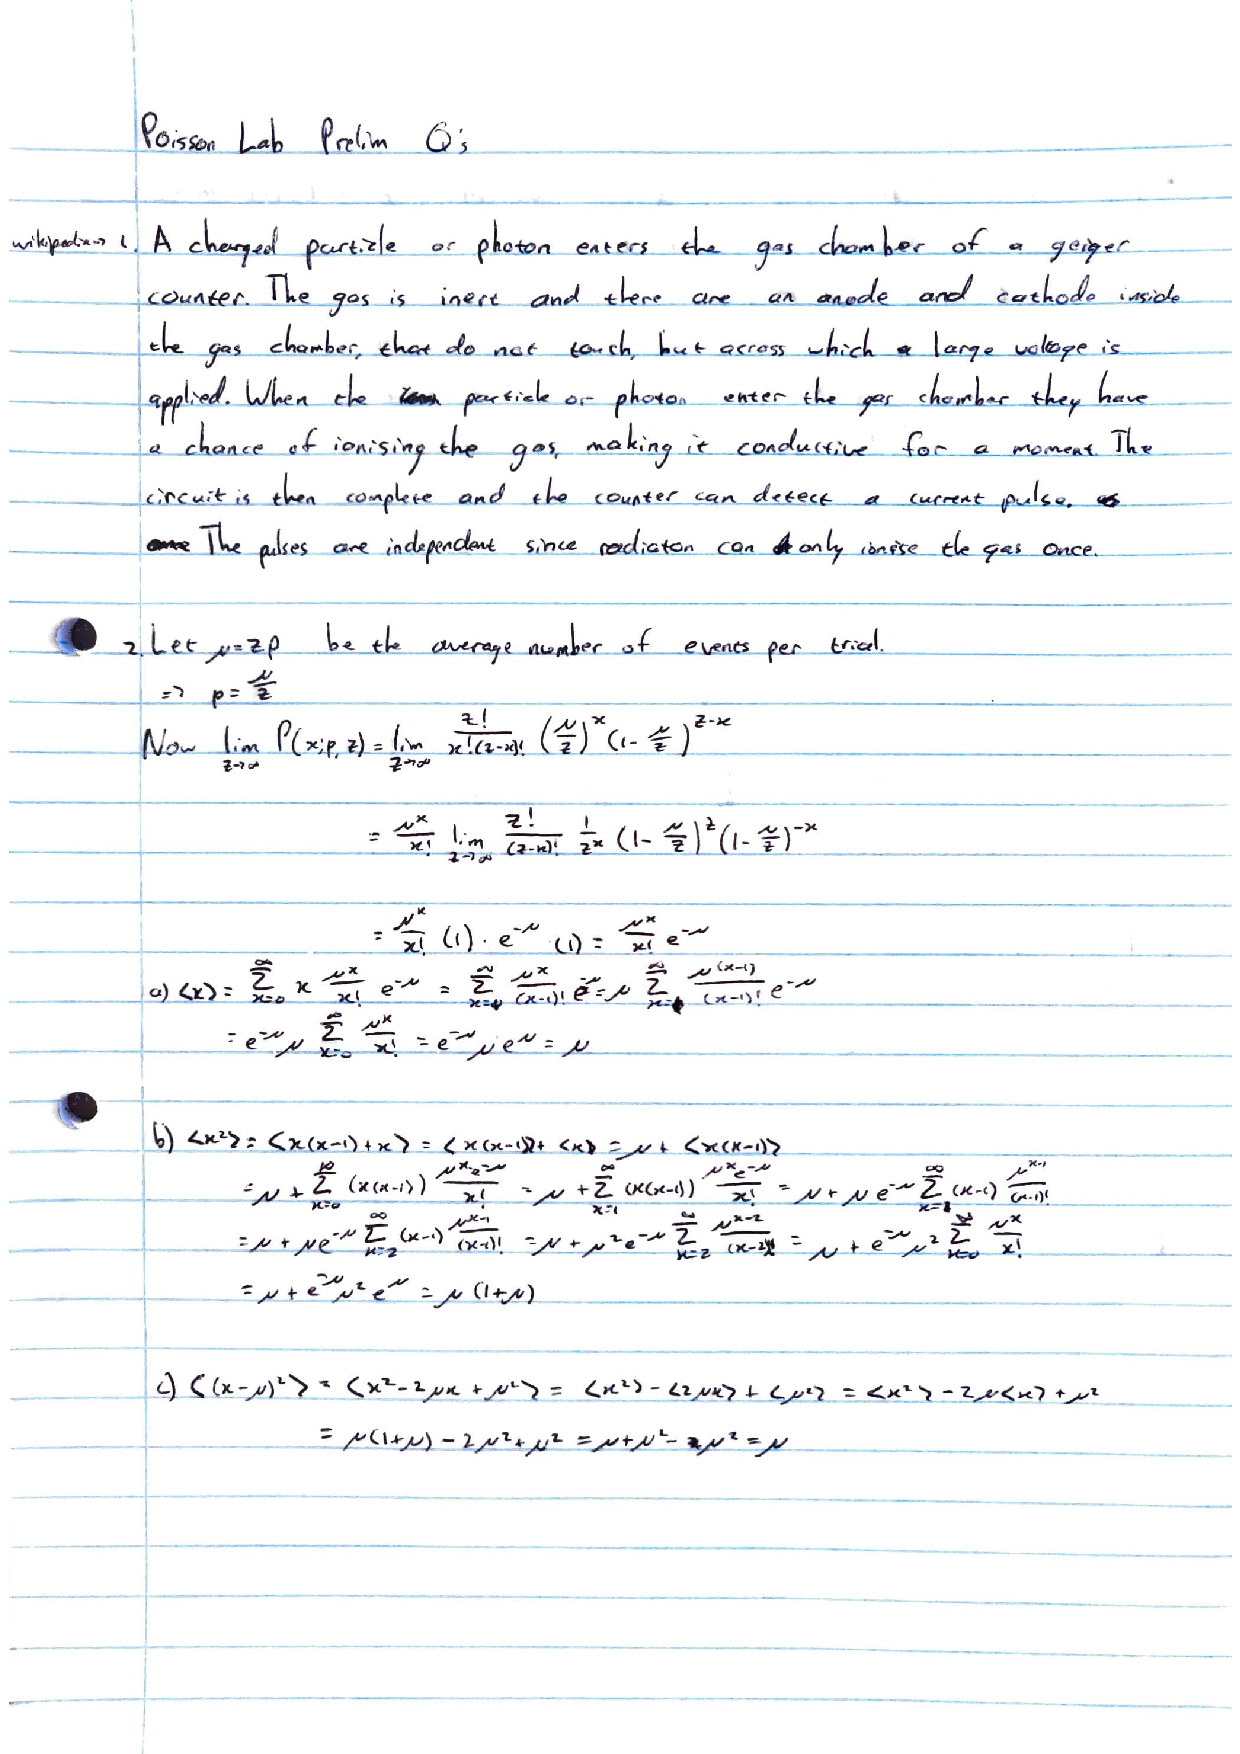
\includepdf[pages=1,scale=0.8,pagecommand=\section{Pre-Lab Questions}\label{app:prelab}]{PrelabQs.pdf}
\includepdf[pages=2-,scale=0.8]{PrelabQs.pdf}


\begin{thebibliography}{9}
    \bibitem{manual}
    W.A. Horowitz, \textit{Poisson Statistics}, (UCT, 2021)
    \bibitem{cowan}
    G. Cowan, \textit{Statistical Data Analysis, Ch. 6}, (Oxford Science Publications, 1998)

\end{thebibliography}


\end{document}